\section{Experiments \& Results}
\subsection{Neural Networks}
Matlab's neural network toolbox is used in training process. We selected the performance function to be cross-entropy since it is a standard \cite and training function to be scaled conjugate gradient. 
We used neural networks with different number of hidden neurons and the correlation of neural network's output and phase is not changing significantly with the number of hidden neurons. This experiment is done on third channel of 10 subjects. The boxplot showing results for different number of hidden neurons is given in figure \ref{fig:hidden}. So we decided to use 20 neurons.
\begin{figure}[h!]
	\begin{center}
		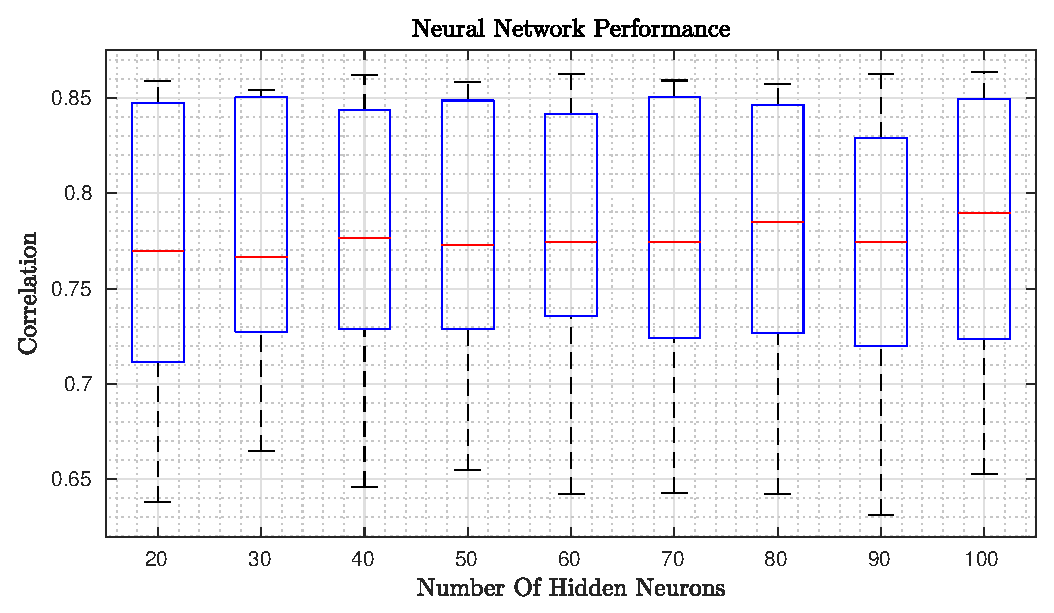
\includegraphics[width=\textwidth]{figures/hidden.eps}
		\caption{Performance of Neural Network vs Number of Hidden Neurons}
		\label{fig:hidden}
	\end{center}
\end{figure}
We measured the performance of neural networks by using correlation measure. The boxplot of correlation between neural network's output and the phase plot is given in \ref{fig:neur_net_corr}. We then corrected the output of neural networks by using the period information, and the result is shown in \ref{fig:neur_net_corr_corrected}.
\paragraph{} In addition to correlation measure we also measured the deviation of detected transition points from real transition points. We introduced a deadband which is equal to 5\% of peak-to-peak voltage around zero before calculating the true transition points.
\begin{table}[h!]
	\centering
	\begin{tabular}{|| c c c c c c c c c c c c c c ||} 
		\hline
		Channel & 1 & 2 & 3 & 4 & 5 & 6 & 7 & 8 & 9 & 10 & 11 & 12 & Average \\ [0.5ex] 
		\hline\hline
		Ins to Exp & 74 & 183 & 76 & 87 & 77 & 74 & 80 & 71 & 146 & 115 & 86 & 82 & 96.8\\ 
		Exp to Ins & 64 & 150 & 66 & 77 & 63 & 67 & 62 & 65 & 126 & 123 & 68 & 65 & 83.2\\
		\hline
	\end{tabular}
	\caption{Deviation From True Transitions in Milliseconds}
	\label{transition_deviation_neural}
\end{table}
\begin{figure}
	\begin{center}
		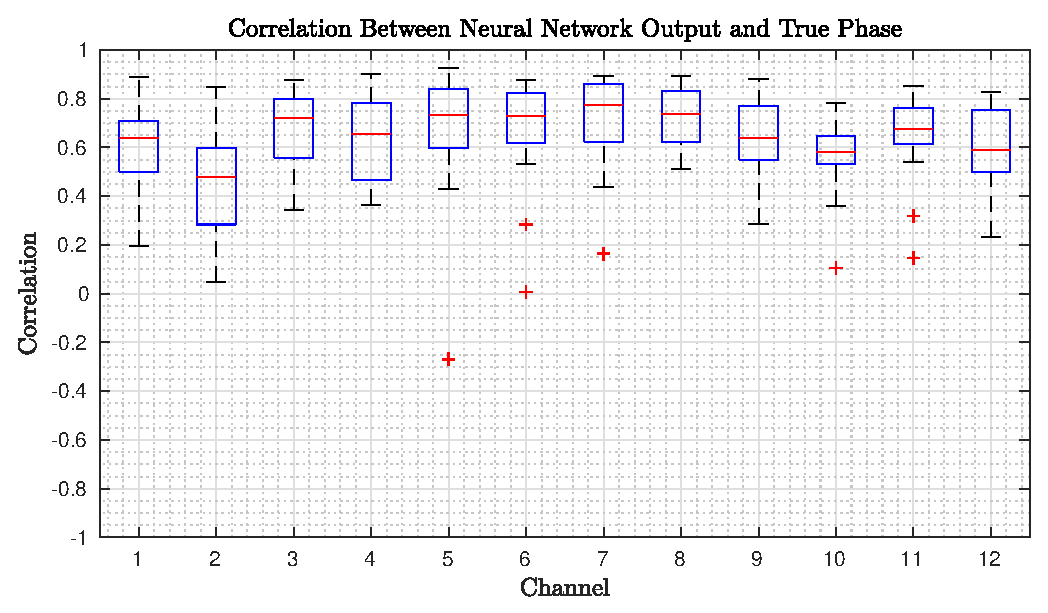
\includegraphics[width=\textwidth]{figures/neur_net_corr.eps}
		\caption{Performance of Neural Network vs Channels}
		\label{fig:neur_net_corr}
	\end{center}
\end{figure}

\begin{figure}
	\begin{center}
		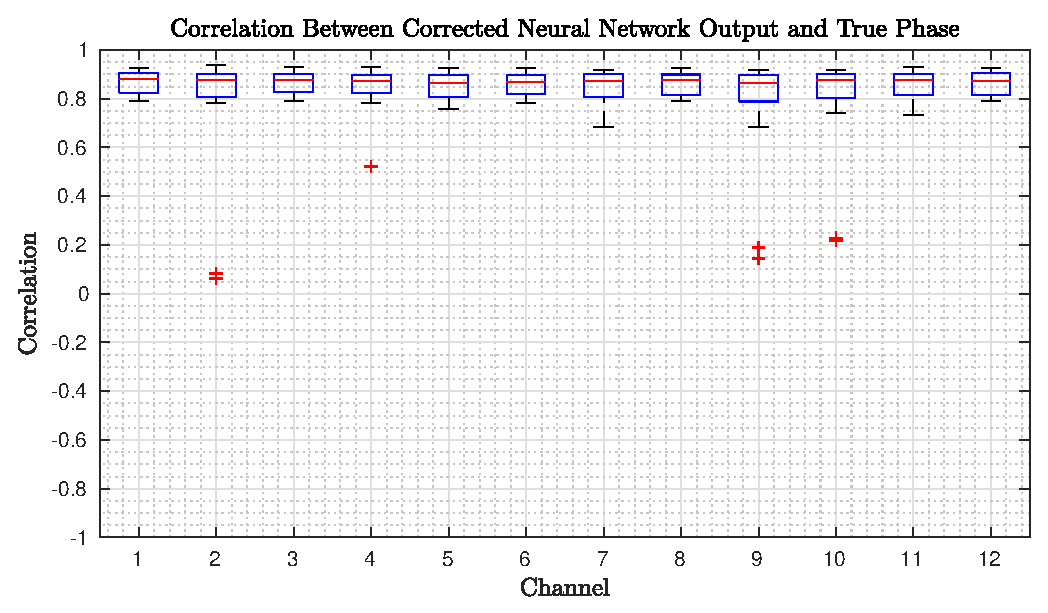
\includegraphics[width=\textwidth]{figures/neur_net_corr_corrected.eps}
		\caption{Performance of Neural Network vs Channels After Correction}
		\label{fig:neur_net_corr_corrected}
	\end{center}
\end{figure}

\subsection{Transition Points Detection Based On Local Minima}
We used first AR coefficient and period information to estimate transition points and calculated the first AR coefficient of the segments between transition points to decide on phase. The correlation between esimated and true flow phase is given in figure \ref{fig:local_minima_phase} and the deviation from true transitions is given in table \ref{transition_deviation_minima}.
\begin{table}[h!]
	\centering
	\begin{tabular}{|| c c c c c c c c c c c c c c ||} 
		\hline
		Channel & 1 & 2 & 3 & 4 & 5 & 6 & 7 & 8 & 9 & 10 & 11 & 12 & Average \\ [0.5ex] 
		\hline\hline
		Ins to Exp & 112 & 121 & 130 & 110 & 96 & 117 & 159 & 102 & 88 & 176 & 110 & 118 & 119.76\\ 
		Exp to Ins & 106 & 186 & 94 & 198 & 113 & 117 & 157 & 149 & 104 & 143 & 131 & 131 & 130.73\\
		\hline
	\end{tabular}
	\caption{Deviation From True Transitions in Milliseconds}
	\label{transition_deviation_minima}
\end{table}

\begin{figure}
	\begin{center}
		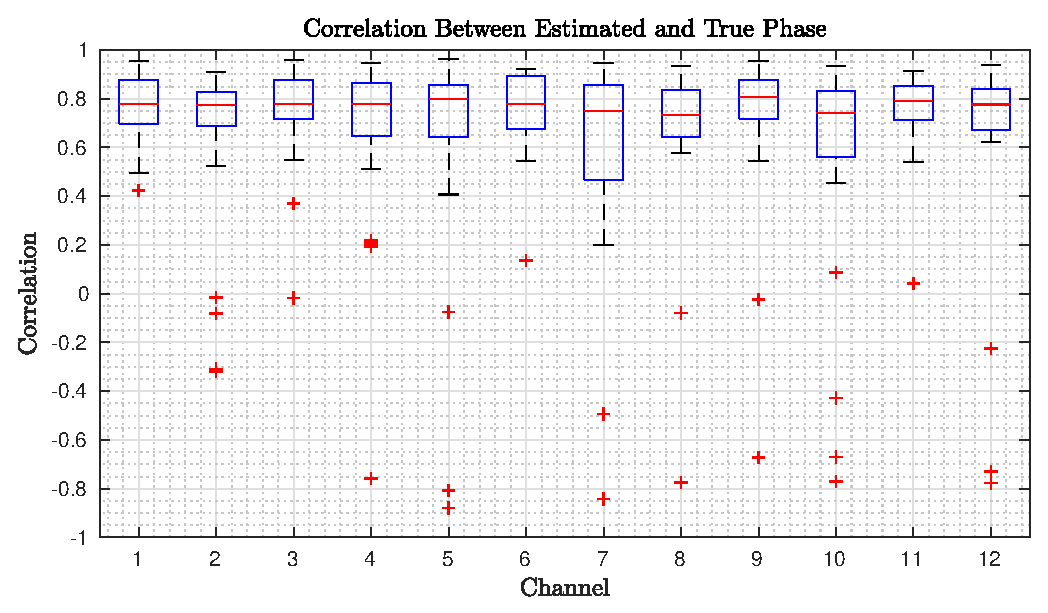
\includegraphics[width=\textwidth]{figures/local_minima_phase.eps}
		\caption{Performance of Phase Estimation Based On Local Minima}
		\label{fig:local_minima_phase}
	\end{center}
\end{figure}